\documentclass{../../sheet}
\renewcommand{\logopath}{../../logos/}

\title{Einrichtungszeug GS-Pool}

\begin{document}
\maketitle
\aufgabe{Anmeldung}
Ihr habt euch wahrscheinlich schon mit eurem Account angemeldet (\texttt{jvk001} - \texttt{jvk080} mit dem Passwort \texttt{jvkws26}). Dateien, die ihr in \texttt{home/jvk\#\#\#/} oder dort in Unterordnern speichert werden im Laufe der Woche erhalten bleiben.
\aufgabe{Die Programmierumgebung (IDE) öffnen}
Wir werden IntelliJ Idea verwenden. Das Programm ist schon auf den PC's hier installiert, ihr müsst es nur öffnen:

\begin{itemize}
	\item Das allgemeine Menu ganz oben links in der Ecke öffnen und Systemwerkzeuge auswählen:\\
	      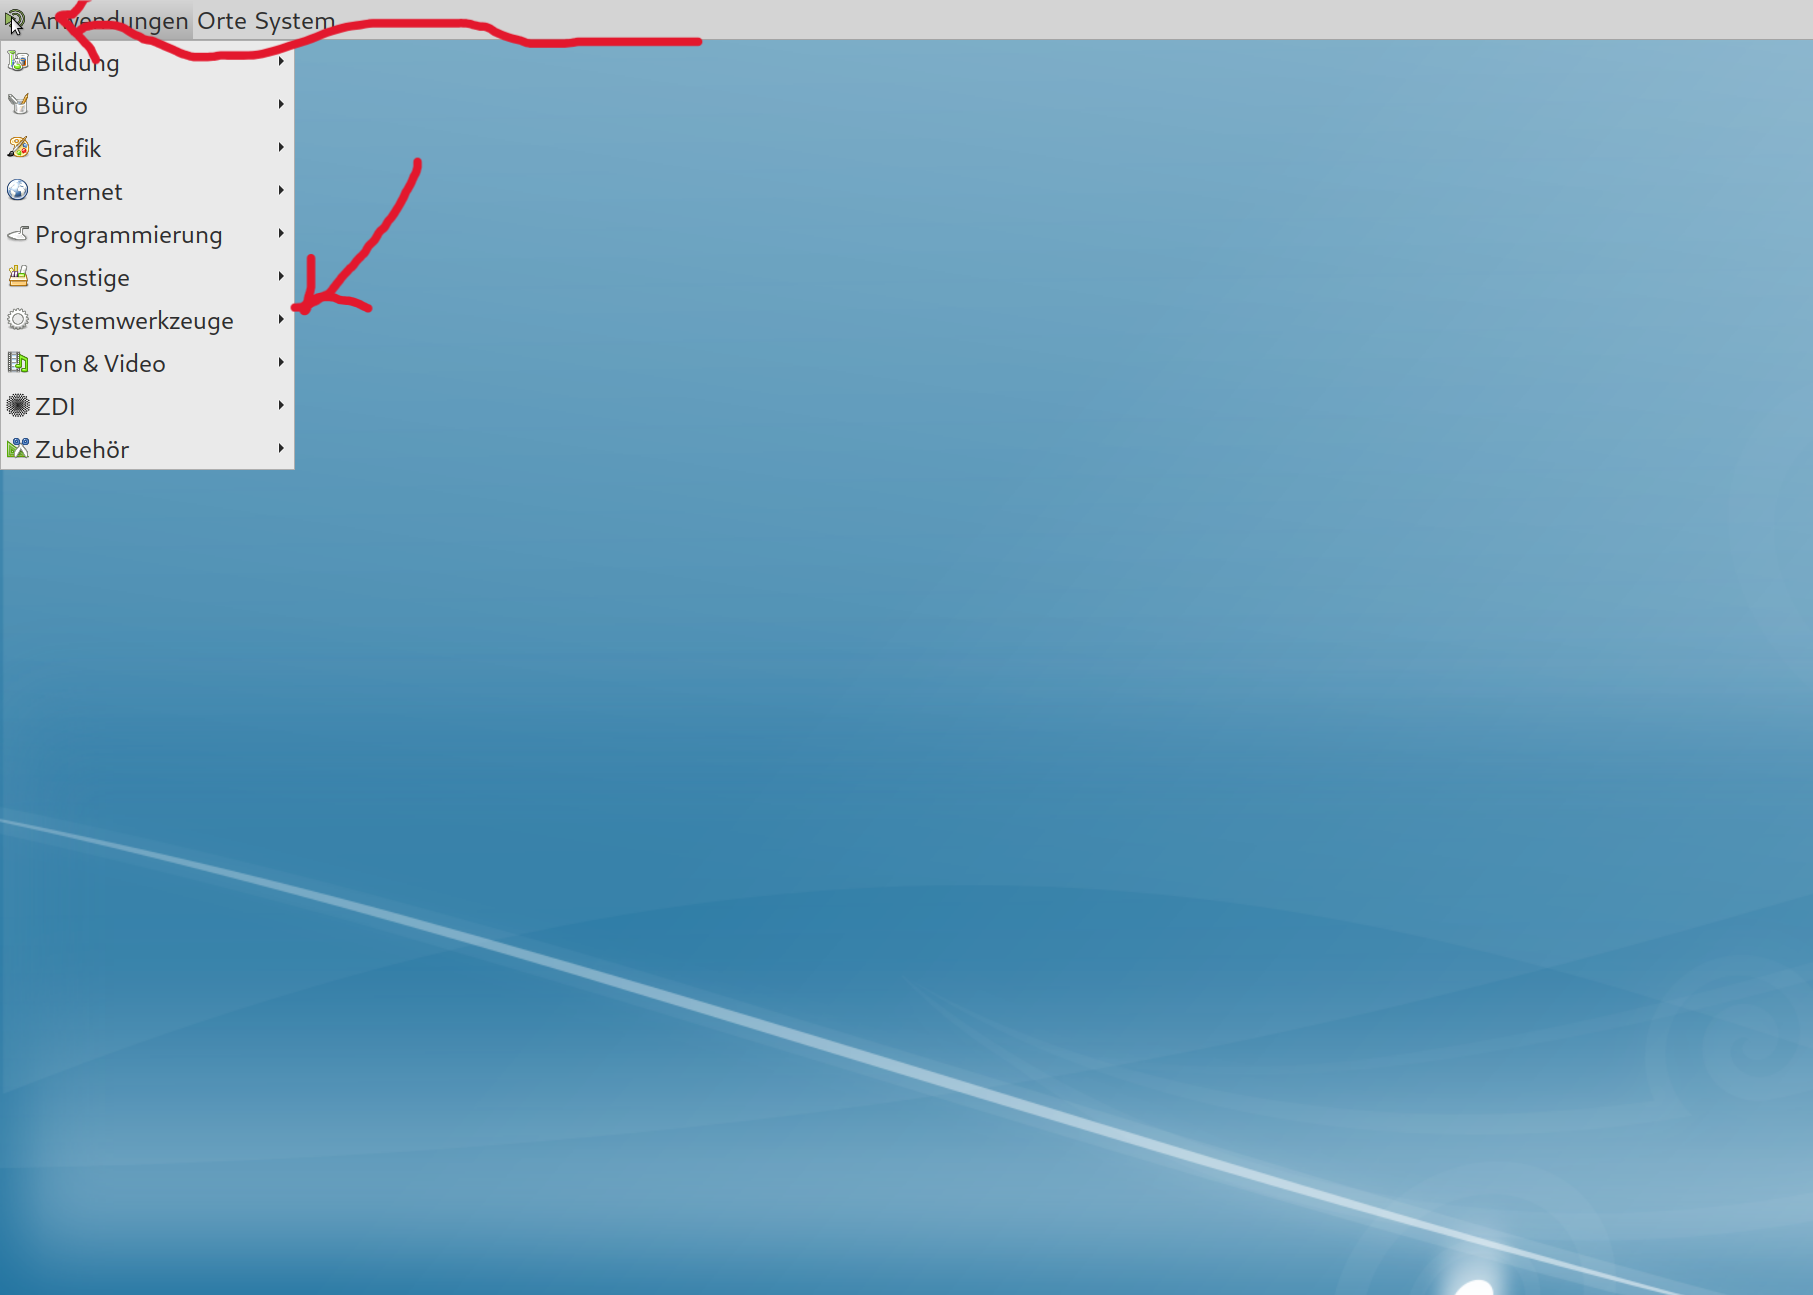
\includegraphics[width=1\linewidth]{../img/pooleinfuehrung01.png}
	      \newpage
	\item Die Konsole öffnen:\\
	      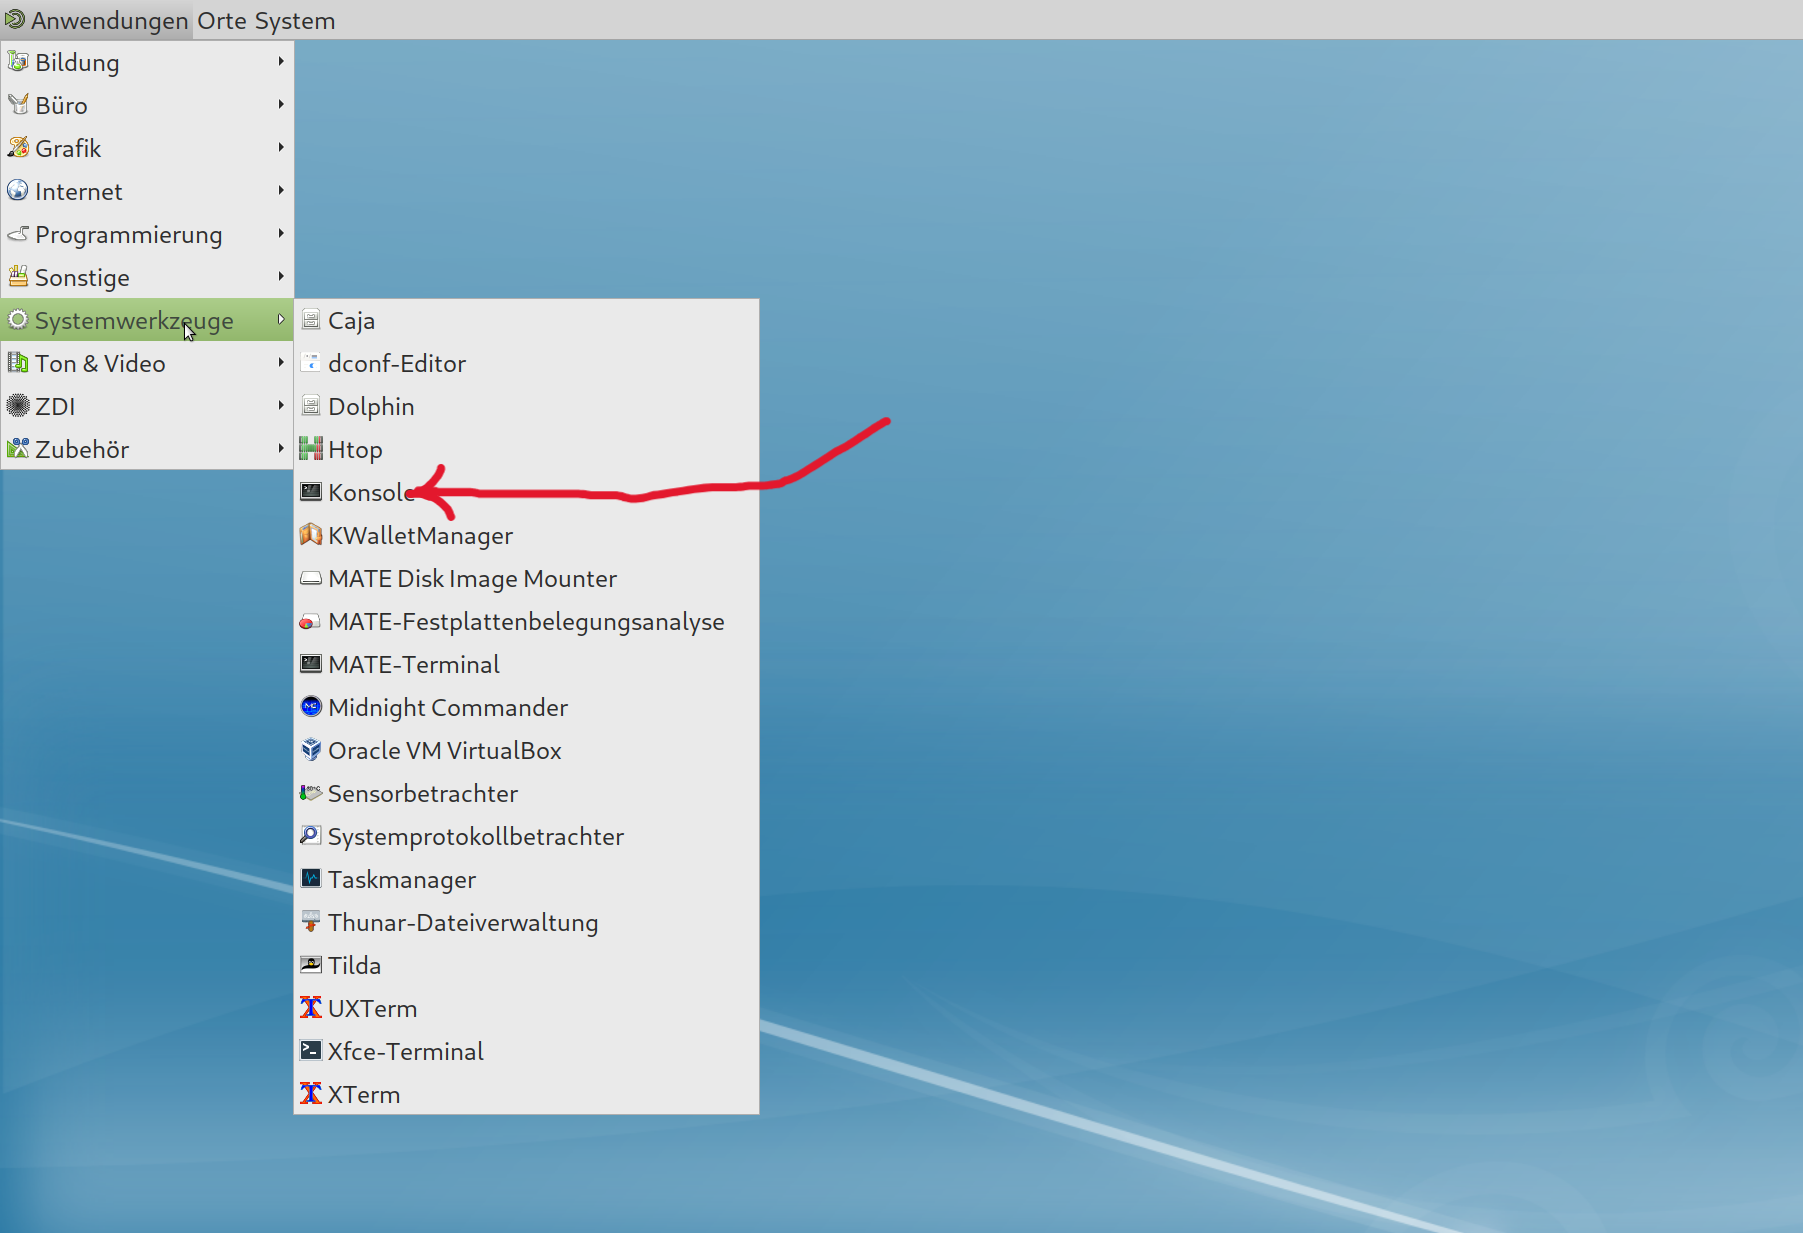
\includegraphics[width=1\linewidth]{../img/pooleinfuehrung02.png}
	\item Mit dem \texttt{idea} Befehl, IntelliJ Idea öffnen:\\
	      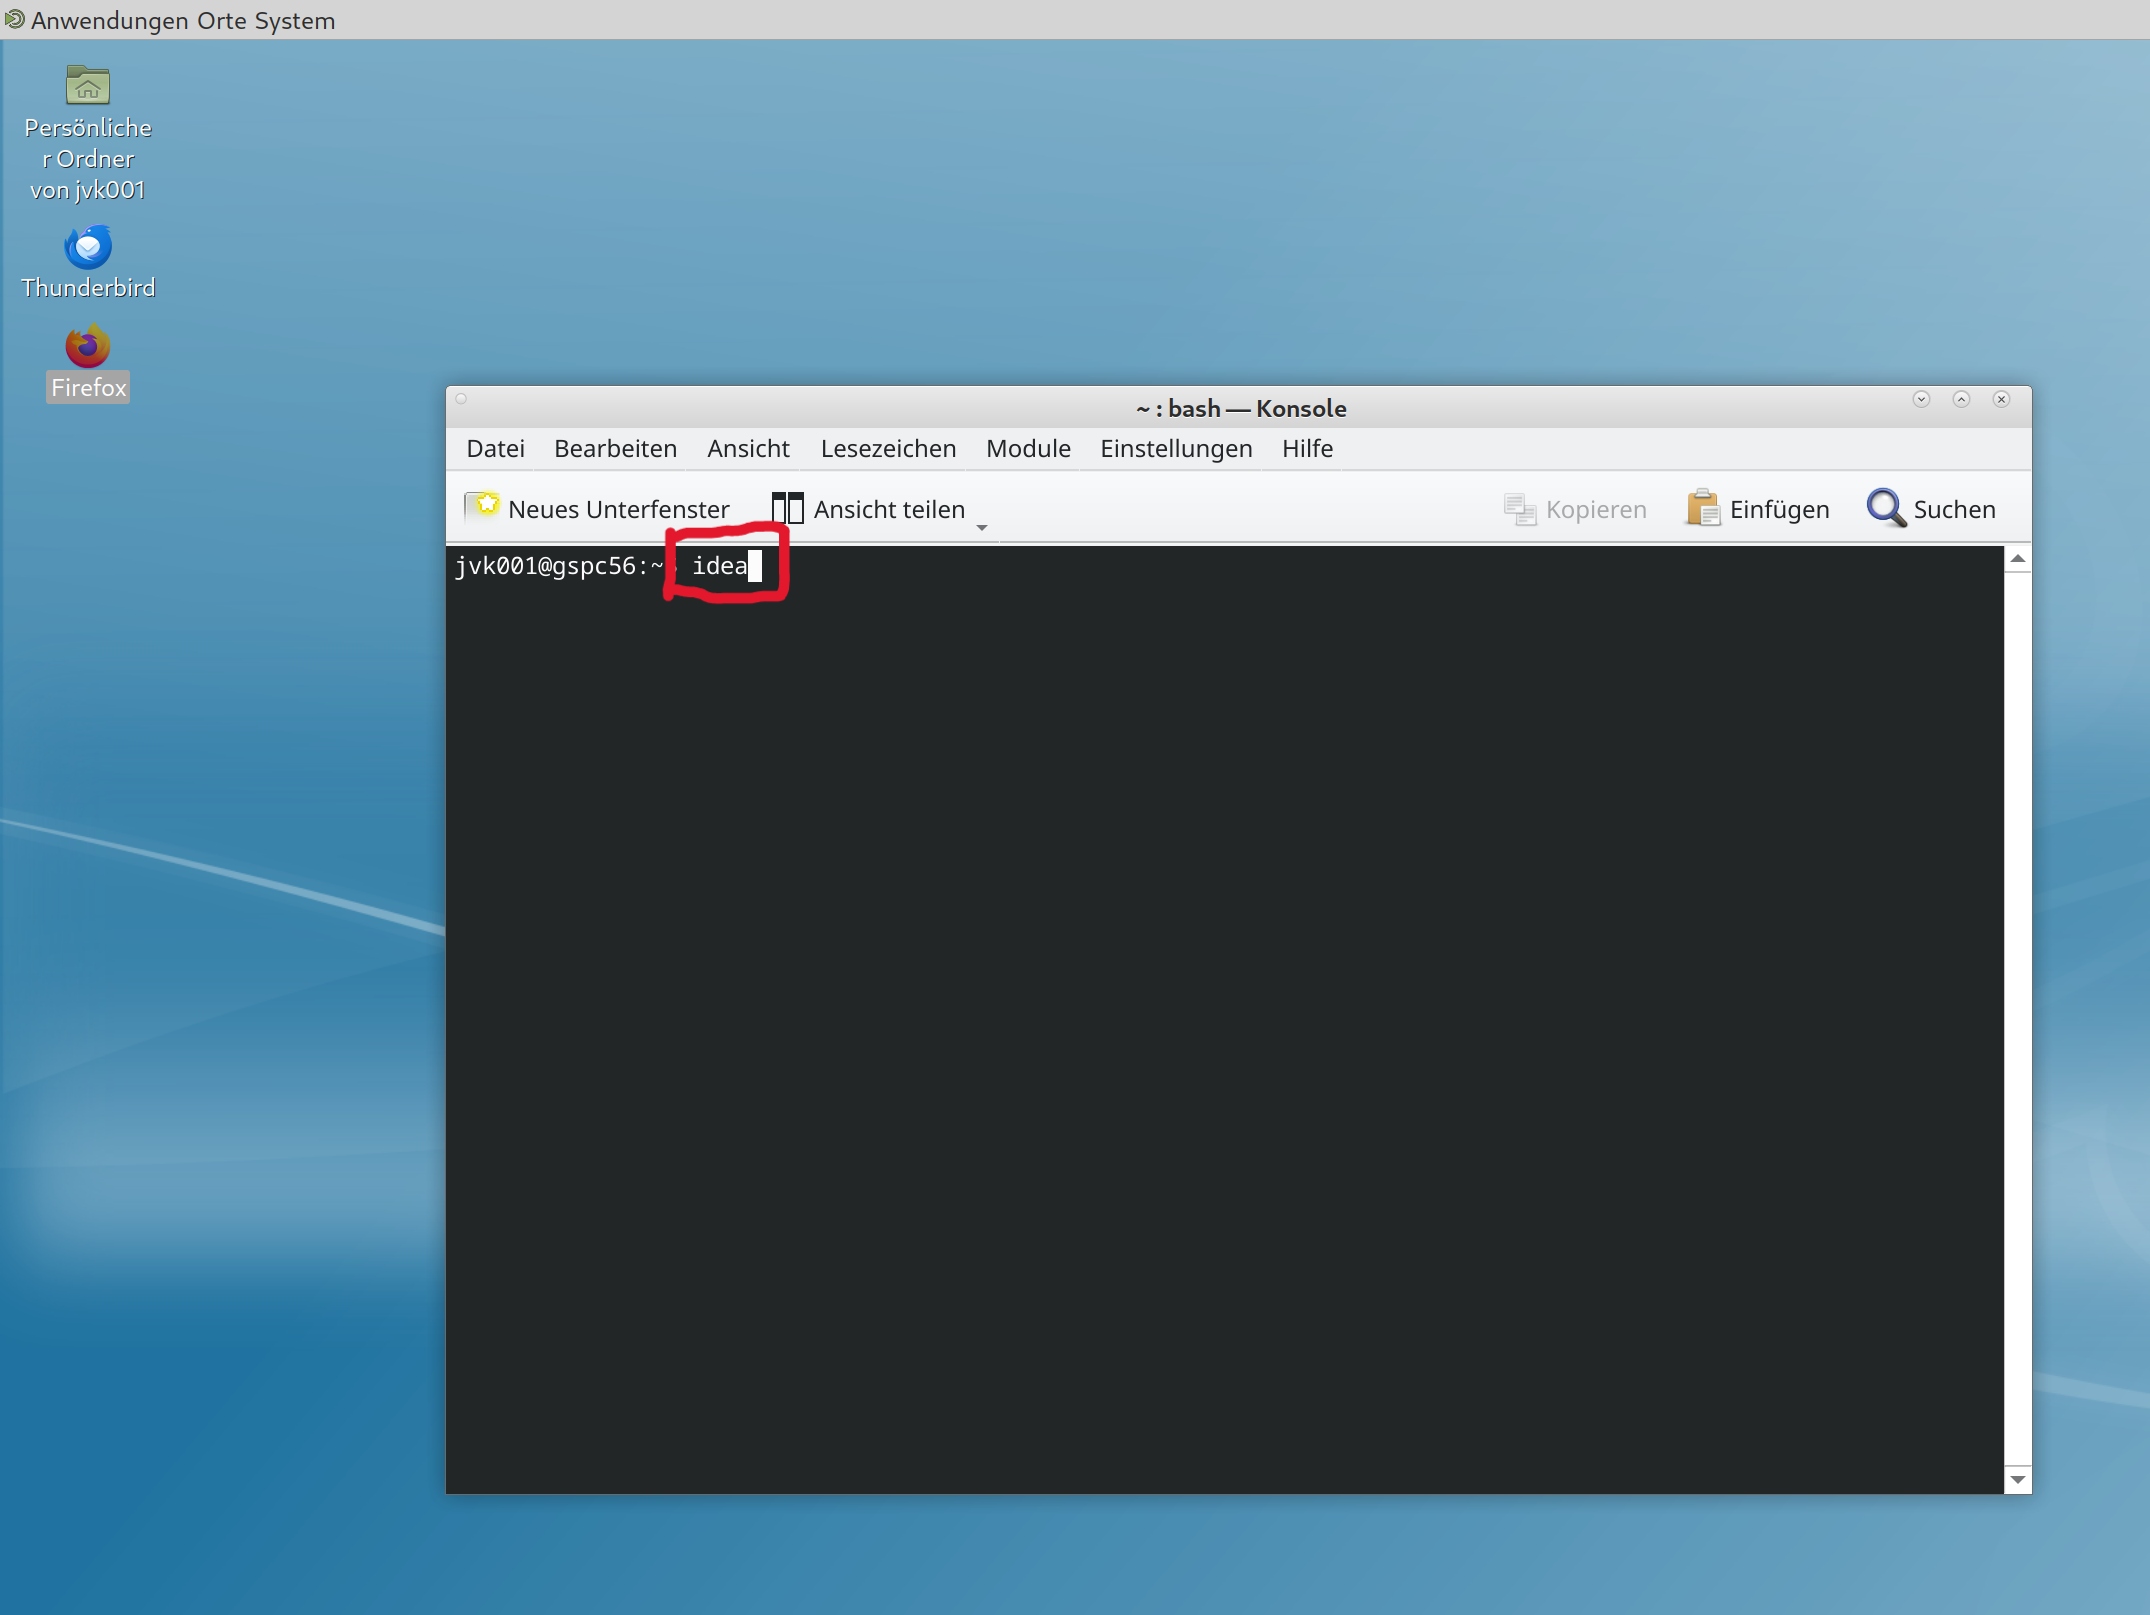
\includegraphics[width=1\linewidth]{../img/pooleinfuehrung03.png}
	      \newpage
	\item Es sollte jetzt gleich so aussehen:\\
	      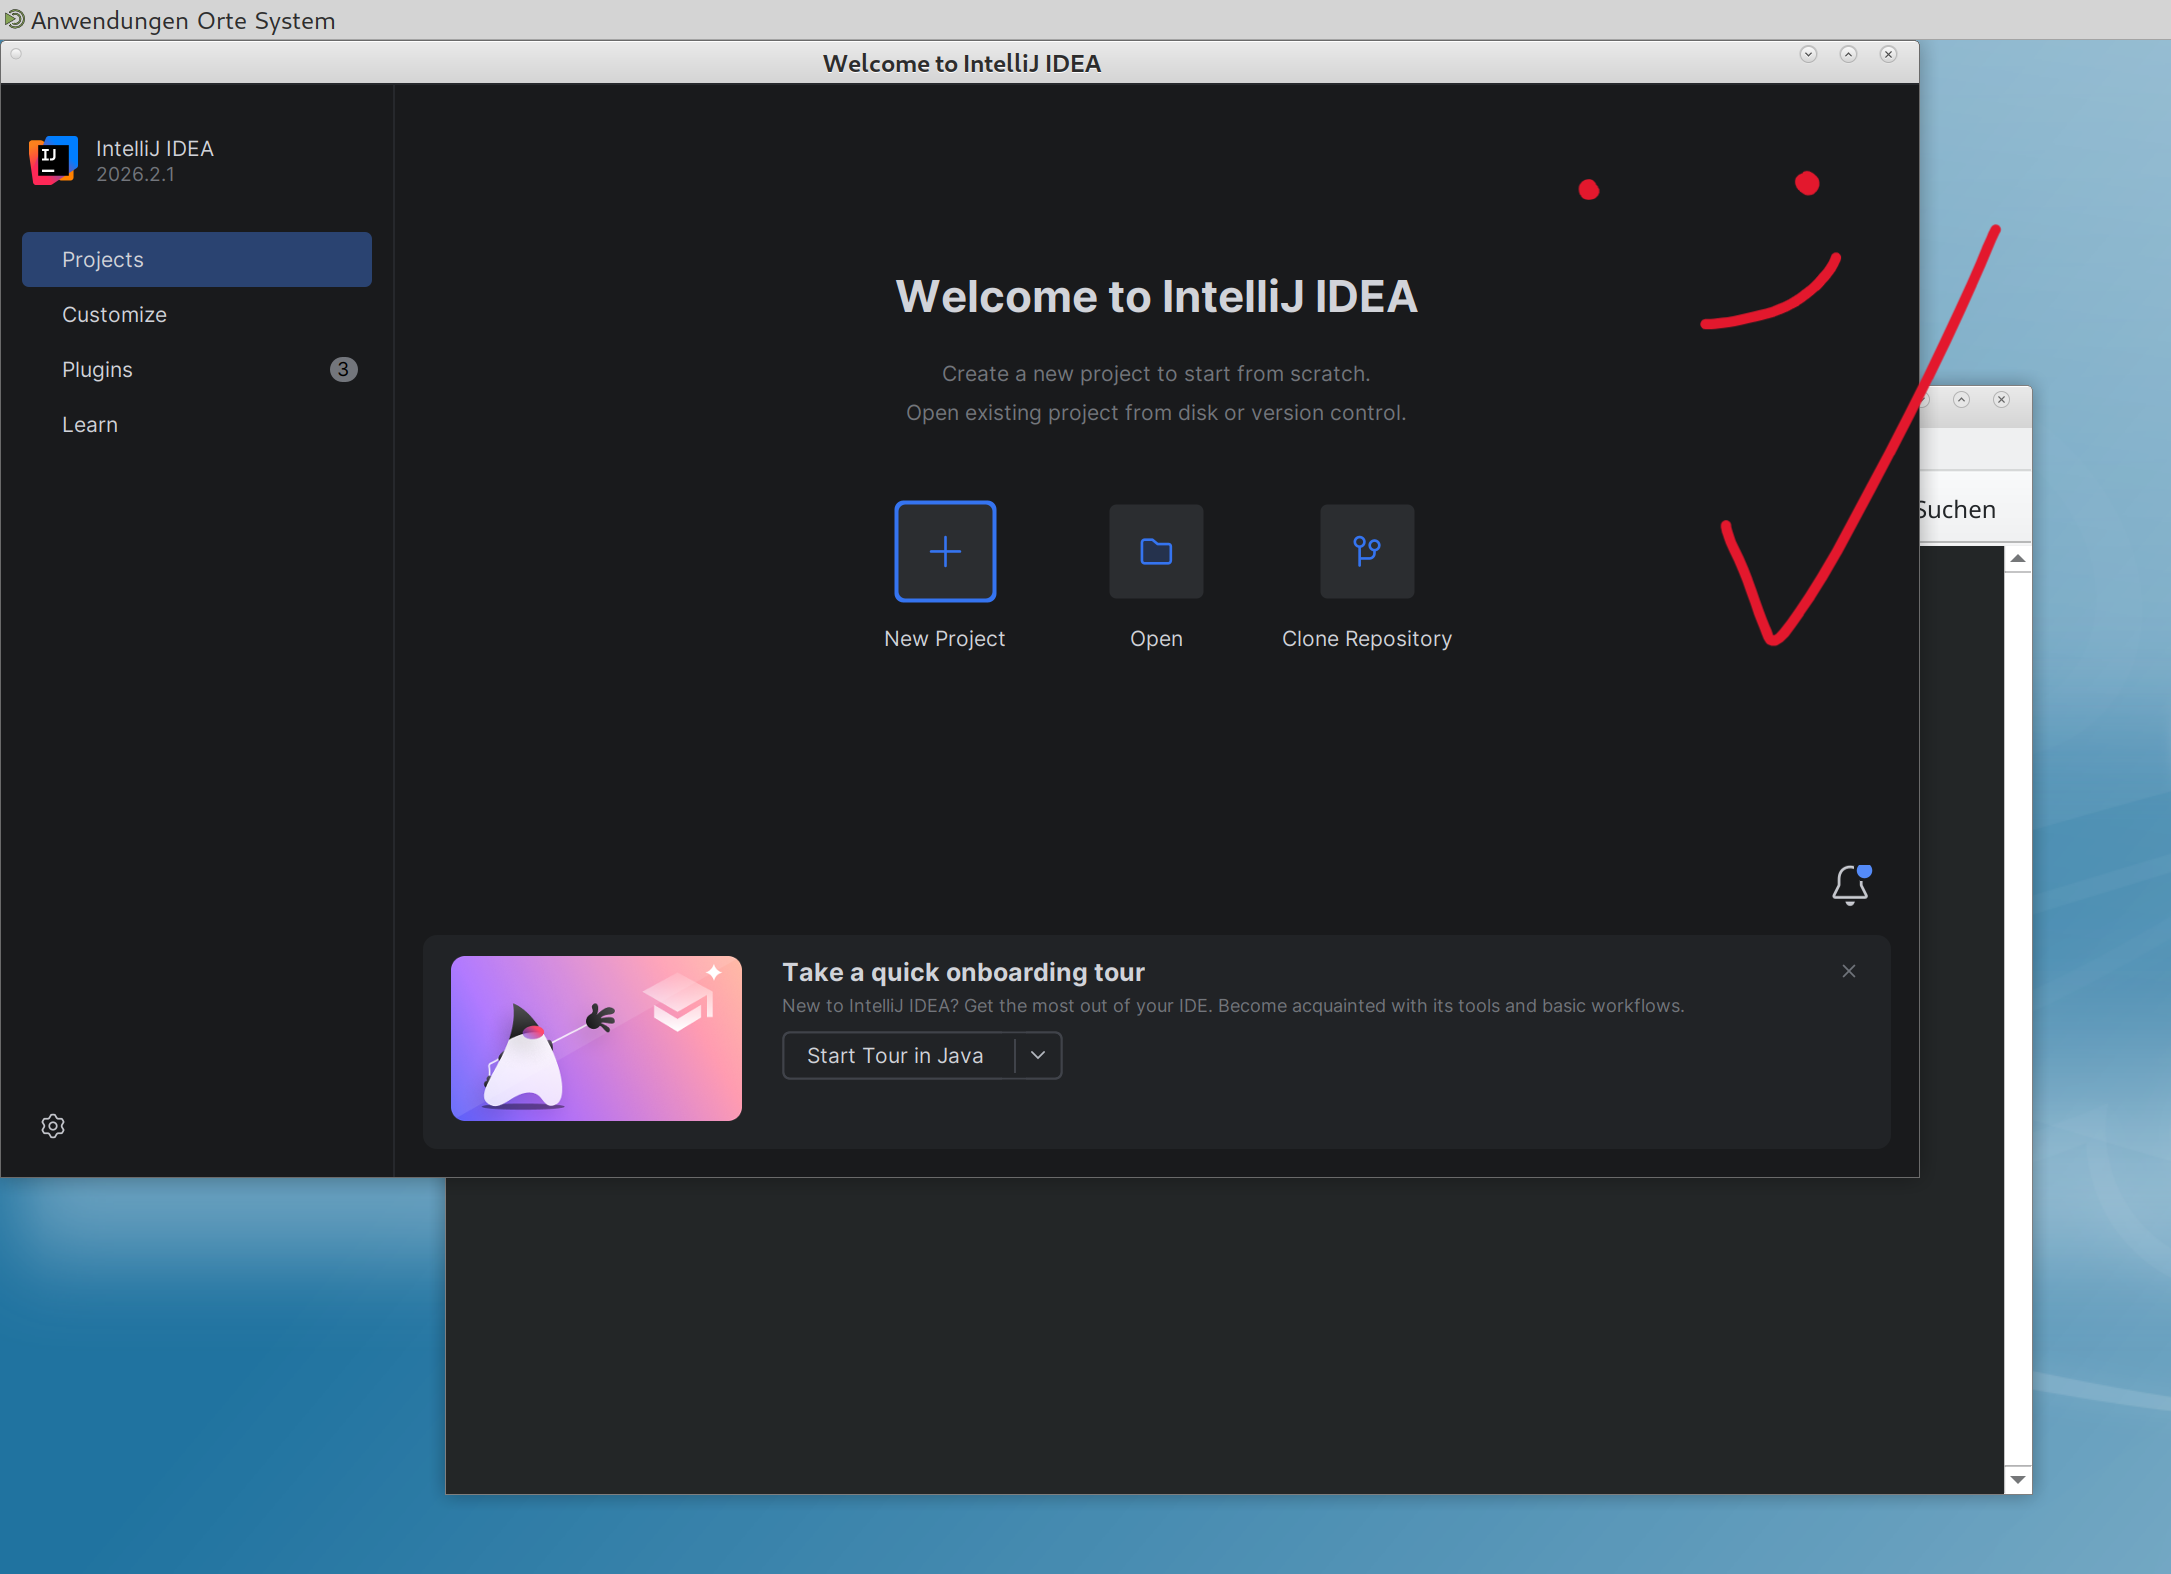
\includegraphics[width=1\linewidth]{../img/pooleinfuehrung04.png}
\end{itemize}



\includegraphics[width=1\linewidth]{../img/memeIDE.jpg}

\newpage





\aufgabe{JDK - Installation}
Wir benötigen ein JDK (Java Development Kit), um Java Programme zu schreiben und
auszuführen.
\begin{itemize}
	\item IntelliJ öffnen \newline \achtung{} Für Pool PCs: Konsole öffnen und \texttt{idea} eingeben
	\item File/Datei gehen oben links in der Menüleiste
	\item Auf \texttt{Project Structure} klicken
	\item Dann auf \texttt{SDKs}
	\item Dann auf das '+' Symbol klicken und auf \texttt{Download JDK}
	\item OpenJDK Version 21 verwenden
	\item Microsoft OpenJDK als Anbieter/Vendor auswählen
	\item Speicherort auswählen (Standardpfad sollte reichen)
\end{itemize}

\newpage

\aufgabe{Projekt erstellen}
\begin{itemize}
	\item In IntelliJ auf neues Projekt erstellen/ New Project klicken
	\item Java auswählen und das Projekt firstProjekt nennen
	\item Nun nen geeigneten Speicher Ort auswählen Achtung: KEIN Git Repository erstellen
	\item Als Build System IntelliJ verwenden und als JDK unsere derzeitig heruntergeladene 21 auswählen
	\item Wir wollen keinen Sample Code
\end{itemize}

Es sollte nun so bei euch aussehen:

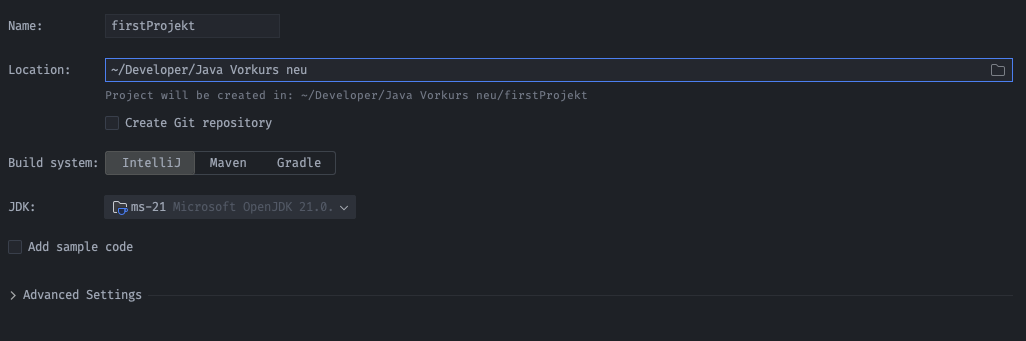
\includegraphics[width=1\linewidth]{../img/projektCreation.png}

\begin{itemize}
	\item Nun auf Create klicken und das Projekt wird erstellt
	\item Nun links in der Projektansicht auf src rechtsklicken und eine neue Java Klasse erstellen
	\item Diese Klasse Main nennen und auf Enter drücken
	\item Nun sollte sich eine neue Datei öffnen, in der wir unseren Code schreiben
\end{itemize}

\aufgabe{Erste Java Klasse}
Nun schreiben wir folgenden Code in die Main Klasse rein
\begin{minted}[fontsize=\Large, linenos=false]{java}
    public class Main {
      public static void main(String[] args) {
        System.out.println("Hallo Welt!");
      }
    }
  \end{minted}


\end{document}